\renewcommand\refname{Literaturverzeichnis}
\addcontentsline{toc}{section}{Literaturverzeichnis}
\printbibliography
\cleardoublepage
\listoffigures

\appendix
\clearpage
\section{Aufgabenstellung}\label{sec:aufgabenstellung}
\begin{figure}[h]
    \centering
    \begin{minipage}[b]{0.75\textwidth}
        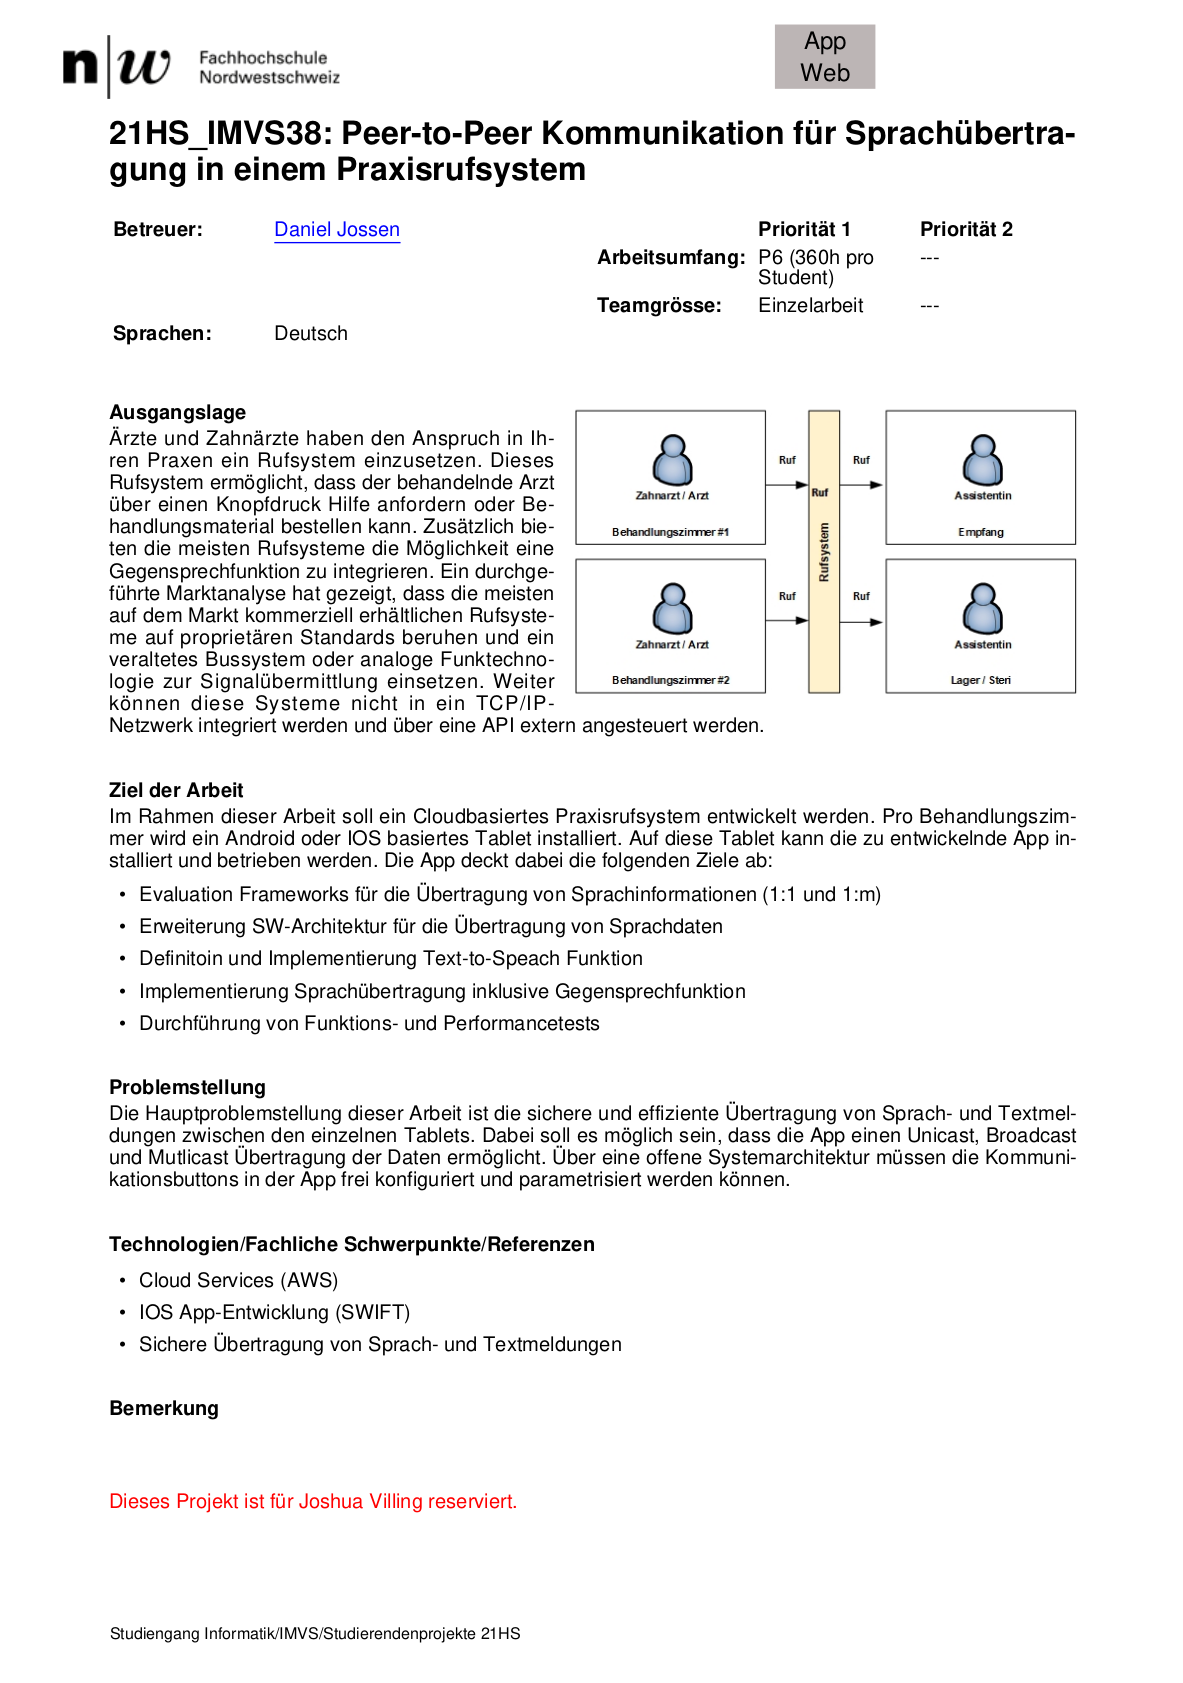
\includegraphics[width=\textwidth]{graphics/aufgabenstellung}
        \caption{Aufgabenstellung}
    \end{minipage}\label{fig:aufgabenstellung}
\end{figure}

\clearpage

\section{Quellcode}\label{sec:quellcode}

Sämtlicher Quellcode der im Rahmen des Projektes entsteht, wurde mit Git verwaltet. Der Quellcode ist für Berechtigte unter github.com einsehbar\footnote{\url{https://github.com/users/jsvilling/projects/3}}.
Berechtigungen können bei Joshua Villing angefordert werden.

\clearpage

\section{Ehrlichkeitserklärung}

«Hiermit erkläre ich, die vorliegende Projektarbeit IP6 - Cloudbasiertes Praxisrufsystem selbständig und nur unter Benutzung der angegebenen Quellen verfasst zu haben.
Die wörtlich oder inhaltlich aus den aufgeführten Quellen entnommenen Stellen sind in der Arbeit als Zitat bzw. Paraphrase kenntlich gemacht.
Diese Projektarbeit ist noch nicht veröffentlicht worden.
Sie ist somit weder anderen Interessierten zugänglich gemacht noch einer anderen Prüfungsbehörde vorgelegt worden.»

\begin{tabbing}
    \\
    \\
    \\
    Left \= Middle \=  \= Right \kill
    Name \> \> \>    Joshua Villing\\
    Ort \> \> \>    Aarau \\
    Datum \> \> \>    01.03.2022\\
    \\
    Unterschrift \> \> \>     ............................\\

\end{tabbing}


